%included in thesis.tex,


\chapter{Background and Literature Study}
This chapter will try to outline the basics needed to understand this report. Mathematical
knowledge are crucial to understand the principles used in robot navigation and decision
making. 


\section{Basics}

\subsection{Reference Frames}
	Movement must be described relative to something. This is the task of the reference systems. There are
	4 important reference system. The ECI (Earth Centre Inertial) which is a truly inertial reference
	frame, i.e. it is not accelerating. Its axis are pointing through the north pole and through the
	equatorial line of the Earth, fixed toward stationary points in space. The centre is as the name
	suggests in the centre of the Earth. 
	
	ECEF (Earth-Centre Earth-Fixed) is another reference frame. It is defined same as the ECI coordinate
	system, but the axis are rotating with the same rate as the Earths rotation rate. This means that this frame
	is not
	strictly inertial, but the angular velocity of the Earths rotation are considered very small, and can
	be neglected compared to other velocities in the same frame. Position on the earth are described by
	\textit{longitude} and \textit{latitude}.

	An important reference frame when considering local motion are the NED (North East Down) frame. This
	frame is defined as the tangent plane on the current position, and moving with the object. The axis
	are pointing towards north, east and down. This frame can be used in local, and small areas, but are
	not valid for intercontinental travel. This frame will primarily be used in this report. 

	The last but important frame are the Body frame, which is the local frame of the object of interest.
	The body frame are defined as the x-axis along its forward movement, y-axis to the right of the
	movement direction, and the last pointing downward, to complete the right-hand system. The
	origin are defined in the Centre of Gravity of the object. This frame are convenient when
	defining velocities, forces and moments. More on reference frames in \cite{fossen} and
    \cite{forsell}.

    The ones which are important in this report is the NED frame, which will be used for
    the global reference frame. The body frame will describe velocities of the robot. But
    theres this last frame which also are very important, that is the \emph{sensor} frame.
    This is where the sensor data are described. Since the sensors are not mounted in the
    centre of gravity of the robot, the sensor data need to be projected into the body
    frame. 

    The dimension of the sensor frame are dependant on the kind of sensor, if its a 2D
    sensor, 3D sensor, or what kind of measurement it gives. This will be described in
    detail later.

    ***********FIGUR AV VERDENEN MED MED KOORDINATSYSTEMER OG LIGNENDE**********
	
\section{Homogeneous Transformation Coordinates}
To represent rotation, translation, shear, scaling in a common matrix representation
homogeneous transformation coordinates are used. In our daily lives we use 3 dimensions.
Homogeneous coordinates uses a four dimensional matrix to represent all of this in one
matrix. This is because matrix representations are fast and effective on computers.



\section{Ranging Techniques}
To determine range to objects are based on some common mathematical principles. They emit
some kind of signal, either light, sound or radio waves, and process the reflected signal.
Some use triangulation to determine the distance, some measure the time-of-flight of the
emitted signal, and some measures the phase-delay of the emitted signal, which actually
just is another way of measuring the time-of-flight. 

This section will first outline the usual range determination techniques then go into the
more specific sensor characteristics in later sections. 


\subsection{Triangulation}
The principle of triangulation is to have two known locations, where the intersection
between two lines from the known locations are the point one wishes to calculate the
location to. 

\begin{figure}[htbp]
    \caption{Triangulation setup}
    \label{fig:triangulation}
\end{figure}


\subsection{Time-of-Flight Measurement}
This is the most widely used range measurement technique. This measures the time taken
when a signal is transmitted to the reflected signal is detected at the receiver. The
signal might be everything from light, to sound, to radio waves. What kind of medium or
signal which is utilized greatly affect the accuracy and errors of the range measurement. 




\section{Project-specific Sensors}
In this section the sensors which have been used in various robot applications will be
discussed and mapped out. The different abilities of the sensors are mapped out, major
error sources are mapped out.


\subsection{2D Sensors}

\subsubsection{Laser Range Finders}


When looking at Laser Range Finder, there are 3 techniques for determining the distance,
\emph{optical triangulation}, \emph{pulse Time-of-Flight} and \emph{frequency modulated
continuous wave} (FMCW). \cite{laser-ranging-critical-review}

\paragraph{Optical Triangulation}
Optical triangulation is performed by using a light source and a placed at known distance
from each other, called the baseline. This is a triangulation setup which
allows for the calculation of the intersection point between the lines. 



This method has some fundamental limits. \cite{laser-ranging-critical-review} 

This technique is mostly used when the measured distance is short and the need for
extremely precise measurements. For example digitalization of 3D objects. 

Not applicable to the project in question


\paragraph{Pulsed Time-of-Flight}
The laser light which is emitted are amplitude modulated, and the received signal is
compared to the emitted signal and the phase delay is measured. This is then directly
proportional to the distance the light traveled. 


\paragraph{Frequency Modulated Continuous Wave}




\subsubsection{Sonar}


\subsubsection{Infrared Sensors and Proximity Sensors}


\subsection{3D Sensors}


\subsubsection{Time-of-Flight Cameras}
This is the article which I'm going to cite. \cite{sr3000}



\subsubsection{Stereo Vision}
Stereo vision is an inexpensive way of finding range measurements. The setup is two or
more cameras some distance away from each other. This distance is called the
\emph{baseline}. The camera images are then compared and a common reference point is
found. The Difference between the images are then used together with the baseline distance
to triangulate the common reference point and then find the distance to the observed
object. 


\paragraph{Pinhole Camera Model}
	The camera properties or parameters can be divided into two categories; \textit{intrinsic} parameters and
	\textit{extrinsic} parameters. The intrinsic parameters are constant parameters and vary from camera to
	camera, and represent the focus distance and image distortion of the pixels located away from the centre of the
	camera image. 
	The extrinsic parameters relate the position of the point relative to camera coordinates. 
	These parameters are of course dependant on the position of the camera and change with time. 	This imply that 
	coordinates of a 2D point in the camera have to be transformed into a 3D point which can be used 
	by the control system. Since 
	we are going from less knowledge about a point to more knowledge about a point, some things are needed to be 
	estimated or measured to gain the ability to solve the 2D to 3D problem exactly.\cite{robotbok}

	Suppose a point in the world reference system, denoted by, $P_w \in \mathbb{R}^3$. The same point
	represented in the camera frame, $P_c$ are related to $P_w$ by a rotation matrix, $\mathbf{R} \in
	SO(3)$. This gives the following equation: 
	\begin{equation}
		P_w = \mathbf{R} P_c + O(t)
	\end{equation}
	where $O(t)$ is the origin of the camera frame. This means that the point in the camera view is
	described by the equation
	\begin{equation}
		\label{eq:ch1-P_c}
        \begin{aligned}
		P_c &= \mathbf{R}^T (P_w - O(t)) \\
		\mathbf{R}^T &= \mathbf{R}^{-1} 
        \end{aligned}
	\end{equation}

	A pinhole camera model are used to capture $P_c$ to image coordinates, $P_i \in
	\mathbb{R}^2$. 
	The principle behind a pinhole camera is that all light beams passes through a
	infinitesmall hole, or point, located in the origin of the camera frame.   
	\begin{figure}[hbtp]
		\centering
		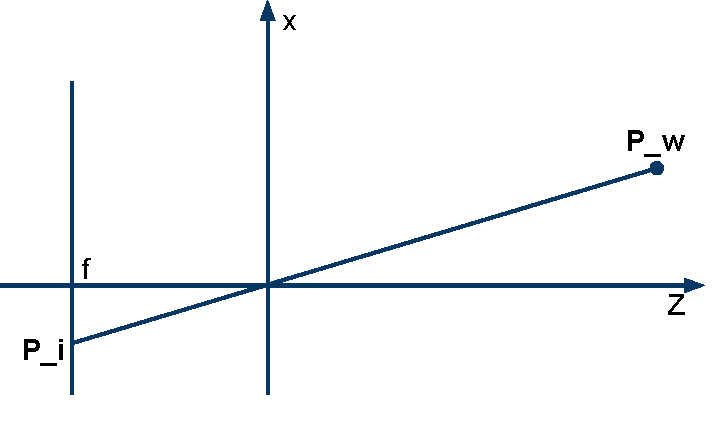
\includegraphics[width=0.5\textwidth]{pics/pinhole_model}
		\caption{Pinhole Camera Model showing two dimensions}
		\label{fig:ch2-pinhole}
	\end{figure}
			
	As seen from Figure \ref{fig:ch2-pinhole} the image plane is located a distance $f$ from the image plane. 
	The point is projected through the hole, and onto the image plane. The principal axis, i.e. the z-axis of the
	camera is pointing
	in the direction of the observed point. For simplicity the image plane is located in the front of the
	pinhole (this is only possible in theoretical case, and would not be possible in a real camera application).
    From this the perspective equations are derived. \cite{robotbok}
	\begin{equation}
		\label{eq:ch2-perspective}
		P_i = \left[ \begin{array}{cc}
					\frac{f}{z_c} & 0 \\
					0	& \frac{f}{z_c} 
				\end{array} \right] 
				\left[ \begin{array}{c}
					x_c \\
					y_c
					\end{array} \right]
	\end{equation}
	The Equation \eqref{eq:ch2-perspective} are the perspective equations, which transforms the observed 
	point into image coordinates. 


\paragraph{Stereo Vision}
    Now suppose we have 2 pinhole cameras located at a known distance $b$ from each other. 
    If we know the focal length, $f$ of both cameras, we can use \emph{triangulation} to
    determine the distance to a common point visible in both cameras. Figure
    \ref{fig:ch2-stereo_geometry} shows the geometry. 
    \begin{figure}[htbp]
        \centering
        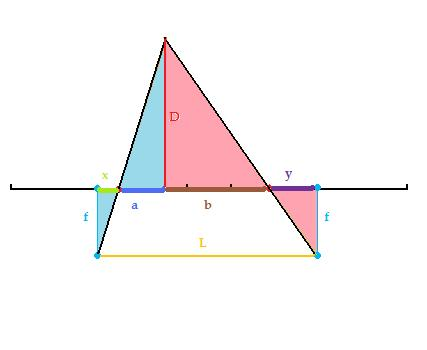
\includegraphics[width=0.5\textwidth]{pics/stereo_geometry}
        \caption{The geometry of stereo vision ****FIKS FIGUR Lag Vektorgrafikk av den****}
        \label{fig:ch2-stereo_geometry}
    \end{figure}

    Distance are inversely proportional to the disparity, and have a clearly nonlinear.
    This means that there are small differences in depth when the disparity is large, and
    when the disparity is small, the variance in depth will be large. This means that the
    depth is more accurate when the object are close to the camera. 
    \begin{figure}[htbp]
        \centering
        \includegraphics[width=0.5\textwidth]{pics/disparity-depth}
        \caption{The relationship between depth and disparity}
        \label{fig:chap2-disparity-depth}
    \end{figure}


    

    The distance to the common point in both cameras can now be calculated by 
    \begin{equation}
        D = f (L / (x+y) - 1)
    \end{equation}
    The value defined by $d = x+y$ is the amount that the object moves in pixels when
    switching from one view to the other. This is called the \emph{disparity}.


\paragraph{Matching}
    To be able to calculate the distance one will need to detect the same point in two
    different images. This is a difficult and a not straight-forward task for a computer.
    Humans are superior when it comes to recognizing objects, but computers are not.

    The process of finding the same point in two images are called matching, and can be
    done in various ways. \cite{gonzalez}

    The matching process is very dependant on features in the environment. If the
    surroundings are featureless the matching becomes very difficult, and the
    probabilities for bad matches are greater. This will cause erroneous distances to the
    objects.




   



\section{Map Data Representation}
The representation of sensor data is important for the functionality of the robot. This is
dependant on the amount of processing power and capacity that is available at the robot.
The area which the robot is to map is also of great importance when choosing the
representation. There are a number of representations that are tried out, and each one has its good and
bad abilities. 

The major representation methods which is used in literature are summarized in the below
sections. There are two major ideas when it comes to map representation, and that is
metric and topological.

Metric representation uses the sensor data as we see it. It is the direct Cartesian
representation of the way the world is. Examples of this are CAD drawings of floor plans
and housing. This maps are often large and inexact, because of many kinds of
uncertainties.

Topological representations uses a more abstract way. The world are represented by graphs,
which is nodes and links between them. This are a sparse and efficient way of representing
the world, but need more processing when the map is built. This kind of maps are not
exact, because they are not expected to be. They simply describe the connection between
different kind of objects, and all objects might have attributes describing how it really
looks. This method is useful in highly structured environments, such as pipelines, sewers,
and office landscapes. This because a series of junctions might tell you where you are
than just the metric information, which might be quite erroneous. 


\subsection{Occupancy Grid Maps}
Occupancy grid maps are a metric approach to the mapping problem and are widely used in 
robotic mapping, mostly because of it is simple to implement and use. It was developed 
by Elfes and Moravec in the mid 1980s, \cite{elfes}, \cite{moravec}. The method is quite 
robust and it is simple to implement with many kinds of sensors. This method assumes that 
the robots pose is known.

This method divides the world into grids with probabilities that the grid is occupied. It
starts with all grids at 50 \%, equal probability that the space is occupied or not. As
the robot moves around it updates the grids according to its sensor readings. When for
example employing laser range finders, the grid at the distance reported from the range
finder are marked as occupied according to some uncertainty set by the accuracy of the
range finder. The grids between the possible detected obstacle will then be decreased
because the probability of obstacles are less. 

Occupancy maps are not the most computationally effective way to represent the world,
especially when it is big. It is cumbersome and may lead to problems when dealing with
cyclic environments. This because of the uncertainty in the sensor measurements and robots
pose and odometry. 


\subsection{Topological Maps}
Object maps are topological maps and represents the sensed world in the form of predefined nodes and links
between them. Each node has a set of attributes, like length, links to doors etc. This is
a compact way to express the world and is much more computationally effective with larger
maps than the occupancy grid maps might be. Examples of such nodes are corridors,
junctions and dead ends, but this nodes must be suited to the application of the robot. 

The problem with this representation is that it needs a lot of input \'a priori. The
operator creates and inputs the map to the robot, which uses this map for navigation. The
largest challenge with this is to make the robot aware of where it is. It needs in some
way to recognize its surroundings, and match it to the \'a priori map.


\subsection{Mixed Approaches}
This is when you take the best of both worlds. The easy and effective way of the metric
maps, and mix them with the abstract topological maps. This will help reduce the size of
the maps in the robots memory, and also make it more computationally effective because the
maps are sparse. 

******?????The mixed approaches are usually not computed on-line***???? (CHECK THIS). This utilizes
the metric approach for the rooms that have a lot of details, chairs, desks etc. and for
corridors and less detailed areas the topological approach, when the metric and
geographical information are not that important. 

This requires lots of processing of the sensor and map data, and should be done off-line
after the robot's mission is finished. 


\section{Sensor Fusion Techniques}
According to \cite{sensor-fusion-mobile-robots} theres a lot of ways to achieve sensor
fusion in mobile robotics. The use of multiple sensors are favorable because the readings
can be fused to make a better estimate of the current situation. 

Multi sensor fusion are widely used in robotics today. This because it allows the designer
to use different measurement principles which have different capabilities. 


\begin{itemize}
    \item Low-level Fusion with unknown statistics
        \begin{itemize}
            \item Rule-based
            \item Geometric and topological maps
        \end{itemize}
    \item Low-level Fusion with known statistics in centralized approaches
        \begin{itemize}
            \item Kalman Filter and probabilistic approaches
        \end{itemize}
    \item Low-level fusion with known statistics in decentralized architectures
        \begin{itemize}
            \item Decentralized probabilistic approaches
        \end{itemize}
    \item High-level Fusion
        \begin{itemize}
            \item Behaviour-based architectures
        \end{itemize}
\end{itemize}


\subsection{Low-level Fusion}
The term low-level fusion is often used when the sensor data is directly integrated
resulting in parameters and state estimates of the model. This methods are mostly purely
mathematical. This method involves the Kalman Filter, and other Bayesian approaches. In
many cases the use of \'a priori information are utilized to verify or improve the
estimates from the sensors.

This methods are probabilistic and requires that you know something about the
statistical properties of the sensors and the \'a priori model. 


\subsection{High-level Fusion}



\subsection{Interpolation Techniques}



\subsection{Probabilistic Techniques}



\section{Feature Extraction}
The need for feature extraction should be obvious when dealing with autonomous robot
navigation. For the robot to know where it is it needs to recognize its surroundings. This
is a difficult step, because computers are not known to be very good at this, as the human
brain is. 

By feature extraction it is meant to recognize one point or feature in one instant and
find the same point at the next time instant. This can be imagined difficult in some
surroundings where theres little individual detail. 

This problem is relaxed a bit when the surroundings are confined to pipelines. The problem
here is that the interior of the pipeline are not rich in detail, and is mostly the same
everywhere the robot travels, except in the different kinds of junctions. By feature
extraction in this report the meaning is to recognize the different types of junctions
that the robot will travel through. 

\cite{theilemann-breivik}




\section{Real World Applications}

Remember MAKRO! The German snake robot used for sewer inspections. 



